\documentclass[conference]{IEEEtran}
\IEEEoverridecommandlockouts
% The preceding line is only needed to identify funding in the first footnote. If that is unneeded, please comment it out.
\usepackage{cite}
\usepackage{amsmath,amssymb,amsfonts}
\usepackage{algorithmic}
\usepackage{graphicx}
\usepackage{textcomp}
\usepackage{xcolor}
\usepackage{multicol}
\def\BibTeX{{\rm B\kern-.05em{\sc i\kern-.025em b}\kern-.08em
    T\kern-.1667em\lower.7ex\hbox{E}\kern-.125emX}}
\begin{document}

\title{A theoretical analysis of the Keep Network random beacon using agent based modeling \\
\thanks{Identify applicable funding agency here. If none, delete this.}
}

\author{\IEEEauthorblockN{Prashanth Irudayaraj}
\IEEEauthorblockA{\textit{Keep Network} \\
prashanth@keep.network}

\and
\IEEEauthorblockN{Antonio Cordozo}
\IEEEauthorblockA{\textit{Keep Network} \\
antonio@keep.network}

\and
\IEEEauthorblockN{Promethea Raschke}
\IEEEauthorblockA{\textit{Keep Network} \\
promethea@keep.network}

\and
\IEEEauthorblockN{Markus Fix}
\IEEEauthorblockA{\textit{Keep Network} \\
markus@keep.network}

\and
\IEEEauthorblockN{Liam Zebedee}
\IEEEauthorblockA{\textit{Keep Network} \\
liam@keep.network}
}

\maketitle

\begin{abstract}
    ABM is an effective tool for analysis of complex systems with long term 
    emergent behavior. In this study we apply ABM to analyse the long term 
    behavior of Keep’s random beacon. We look for the emergence of steady 
    state behavior, at which point we evaluate the sensitivity of specific 
    group and signature characteristics to various parameters. The results 
    of this study illustrates the effectiveness of ABM as an aid to the design 
    of novel distributed systems. 

\end{abstract}

\begin{IEEEkeywords}
Token Engineering, Agent Based Model, Distributed Systems
\end{IEEEkeywords}

\section{Introduction}

\section{Agent Based Modeling (ABM)}
ABM has traditionally been a tool to simulate complex dynamic systems 
such as the spread of pathogens \cite{Bauer2009}, social psychology 
\cite{Smith2007}, and financial markets \cite{Feng2012}. It is well suited
to systems that resist simple analytical solutions due to the interaction of 
complex individual agents with varying attributes. As a bottom up approach, ABM
has been gaining in popularity over tradtional methods such as Discrete Event
Simulation, and can provide more convincing theoretical analysis than approaches
such as general equilibrium analysis \cite{Wang2018}.

The nascent field of token engineering is currently establishing its own set 
of tools and processes. As such, ABM lends itself well to analyzing these systems
to support the design process and evaluate system state after launch.

\section{Analysis of Token based systems}


Discuss the use of ABM for token engineering. Cite recent papers.

Agent based systems could help evaluate trends in behavior related to
various system parameters. They may not however, accurateley represent 
actual system performance. 

Discuss levels of complexity, with citations. Why greater complexity may
not get you much more insight.

\section{Overview of the Keep Random Beacon}
The Keep Network random beacon uses a threshold relay simuliar to the one proposed
by DFINITY and based on the BLS signature scheme \cite{} (NEED CITATION)

\subsection{Role of the model in the design process}
The initial architecture of the Keep beacon was designed by (need input from Antonio)
what purpose did the simulation serve?

\section{Key research questions}
\subsection{When could steady state behavior emerge?}
Emergence of steady state behavior occurs as a confluence of several factors and is difficult
to predict at the design stage. Specifically, process that take several blocks to complete 
such as DKG that often occur asynchronously can create large swings in values such as number of active
groups or percentage of compromised groups. 

\subsection{How could node failures affect system behavior?}
Nodes may go offline or fail entireley. Since their participation in groups is critical to the 
success of the threshold relay, it is important to understand the impact of various levels
of failure on group characteristics. In particular, failures can result in disproportionate ownership
of groups which may cause a byzantine fault to occur. 

\subsection{How could different stake distributions affect system behavior?}
Stake distributions can also skew ownership of groups and can lead to a byzantine fault. A more
centralized distribution could once again lead to a greater ownership of groups by a few entities
thus creating conditions for the group to be compromised. 

\section{Model Creation}

\subsection{Key Terms}
\begin{itemize}
\item Node: A computational entity with memory and computational power sufficient to to run a 
keep client
    
\item Node Owner: may own 1 or more nodes and can allocate different levels of stake to each node
    owned
    
\item Stake: A bond that make a node eligible to participate in a group 
    
\item Group: A collection of nodes who have successfully completed DKG together
    
\item DKG (Distributed Key Generation): The processes of generating keys for each node enabling
    them to sign using Keep's version of Threshold ECDSA \cite{Gennaro2018}.
    
\item Signature: The process of securely generating a random number using Threshold ECDSA \cite{Gennaro2018}
    
\item Ownership Percent: The level of ownership a specific entity has in a group or signature
    
\item Lynchpin: A node who's ownership exceeds the maximum malicious threshold
\end{itemize}

\subsection{Model Structure}
We construct the model using the MESA ABM framework (cite). MESA consists of an agent class with
attributes and methods. We generate 3 types of agents Nodes, Groups, and Signatures. TABLE shows 
the specific differences in each of these.

ADD table for Agent types
\begin{table}[htbp]
    \caption{Node Agent}
    \begin{center}
    \begin{tabular}{|c|c|c|c|}
    \hline
    \textbf{Key Attributes}&\multicolumn{3}{|c|}{\textbf{Node Agent}} \\
    \cline{2-4} 
    \textbf{ } & \textbf{\textit{Node}}& \textbf{\textit{Group}}& \textbf{\textit{Signature}} \\
    \hline
    Connection Delay & X &  &  \\
    Ticket List & X &  &  \\
    Connection Failure Percent & X &  &  \\
    Node Percent & X &  &  \\
    Malicousness & X &  &  \\
    Operator  & X &  &  \\

    \hline
    \multicolumn{4}{l}{$^{\mathrm{a}}$Sample of a Table footnote.}
    \end{tabular}
    \label{table}
    \end{center}
    \end{table}

Decide whether all parameters should be listed?


The simulation model consists of the model class which instantiates the various agents
and steps through the simulation. At each step the state of the model and each agent
is updated. The scheduler manages the sequence of state changes. For this model we use
a simulataneous activation scheduler, which first stages updates for each agent and then 
advances them simultaneously.  (NEED TO CHECK SCHEDULER SEQUENCE AGAIN)

Usually steps measure a change in time. Therefore for our simulation we assume
1 step = 1 block.

\subsection{Runs}
We perform two sets of experiments to answer our research questions. 
\begin{itemize}

\item Single run: Our single run of 1000 steps provide a first look at the 
performance of the sim, quickly. We also use this first experiment to evaluate
when steady state behavior could occur. We also perform some initial evaluations
of the impact of different stake distributions.

\item Multiple runs: The second experiment consists of multiple runs with varying 
parameters. For each change in parameter we perform 6 runs. By varying parameters 
in these runs we attempt to identify sensitivity. We measure this sensitivity after
the start of steady state behavior which we identify in the single run. 
    
\end{itemize}

\subsection{Assumptions}

\textit{Stochastic Assumptions}

To simplify the model we make stochastic assumptions for exogenous processes.

\begin{itemize}

\item Node Connection Delay: We apply a random uniform distribution to a user specified range (NEED JUSTIFICATION OR A JUSTIFIED SAMPLING)
\item Node Connection Failure: This is one of the parameters we intend to adjust to test for sensitivity. Therefore we
randomly pick a percentage of nodes to fail using a uniform distribution.
\item Node Death: We uniform randomly pick nodes to die at a user specified rate.
\item Signature Delay: A delay between when a signature is triggered and when it is executed. We use a poisson distribution. (NEED JUSTIFICATION or REFERENCE)
\item Node Owner Assignment: We use a normal distribution to assign owners to nodes. (NEED JUSTIFICATION)
\end{itemize}

\textit{Stake distribution} 

Since one of our research questions involves understanding the effects of centralization
on system behavior, we use three different token distribution models with 
varying degrees of decentraliation to evaluate this impact. 

\begin{itemize}
\item Linear Distribution: We assume a simple linear distribution as our most 
decentralized case. We take 50000 stakes and allocate them linearly to 100 nodes
as shown in Figure \ref{fig:linear_distribution}

\begin{figure}
    \includegraphics[width=\linewidth]{linear.png}
    \caption{Linear Stage Distribution}
    \label{fig:linear_distribution}
\end{figure}

\item Ethereum Distribution: In the spectrum of decentralization, we assume 
ETH to be moderateley decentralized. We therefore take the distribution of the 
top 30 percent account holders and apply it with some normalization in Figure \ref{fig:eth_distribution}.
(NEED TO JUSTIFY TOP 30 PERCENT)

\begin{figure}
    \includegraphics[width=\linewidth]{eth_distribution.png}
    \caption{Top 30 Percent Ethereum Distribution}
    \label{fig:eth_distribution}
\end{figure}

\item Assumed Stake Distribution: Should we disclose?
\end{itemize}


Assumptions
Model Assumptions
    
\section{Verification and Validation}
Benchmark using analytical methods - from Promethea

\section{Results}
\subsection{Emergence of steady state behavior}
Using the single run experiment, we discover that system consistently appears to 
stabalizes to steady state usually around 400 blocks, and usually due to normalization of bootstrapping states. 
However, final steady state values for the percentage of total groups that are compromised
appears to vary significantly and is dependent on the degree of concentration in the 
stake distribution. 

\subsection{Convergence pressures}

The model primarily converges to steady state due to factors such as
signature request frequency, node availability, and group creation/expiration. We discuss a few
steady state values of interest.

\textit{Active group count} Groups are generated with every request, and intially
during the bootstrap phase a set number of groups are generated with available nodes. In the current
simulation, requests are generated as coin tosses (binomial) at each step. The steady state number of 
active groups is a function of number of new requests and rate of group expiry. In the current setup, 
we see the number of active groups converging to 15 after 400 blocks.

\textit{Percent Compromised Groups} For concentrated distributions such as Ethereum, the steady state level of compromised
groups appears to vary between 0-100 percent (SHOW), with a tendancy to be either close
to 0 or close to 100. For distributions with greater spread, such as our hypothetical linear
distribution, we see steady steat levels within the 50-80 percent band for the given set
of parameters (NOTE PARAMETER SETTINGS) \ref{fig:steady_state}. We expect a similar band but at
different parameter levels for different parameter settings. (CHECK THIS AGAIN)

\textit{Percent Lynchpinned Signatures}

\subsection{Effects of Node failures on group and signature characteristics}
To evaluate the possible effects of node failure on group and signature characteristics, we use the
multi-run study. We then observe trends in the specific parameters discussed below.


\subsection{Effects of stake distributions on group and signature characteristics}


\section{Conclusion and Future work}
\begin{itemize}
\item Dynamic systems -Transfer functions instead of stochastic representations?
\item Utility functions
\item Genetic Algorithms
\item Additional questions
\end{itemize}

\bibliographystyle{plain}
\bibliography{Simulation_paper.bib}

\begin{figure*}[h]
    \onecolumn
    \centering
    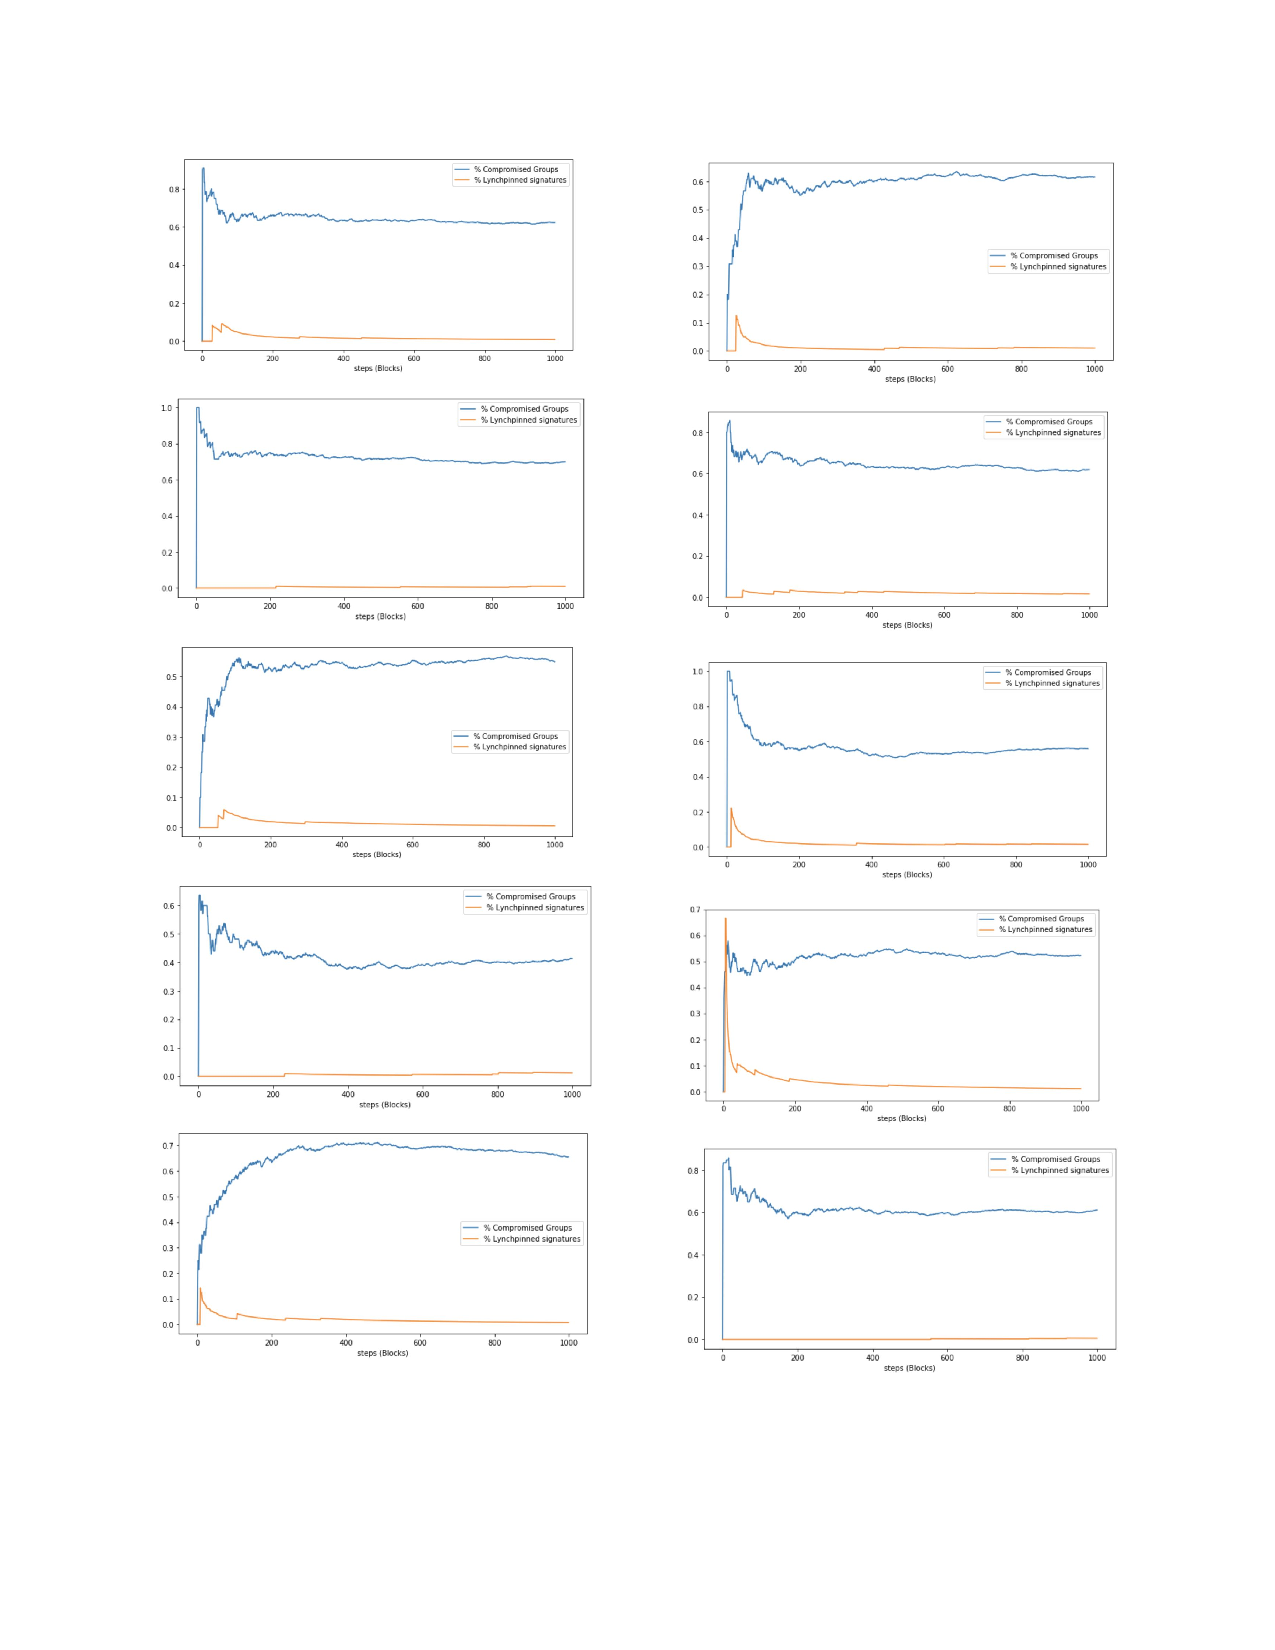
\includegraphics[width=\linewidth]{steady_state_behavior.pdf}
    \caption{Emergence of Steady State Behavior}
    \label{fig:steady_state}
\end{figure*}

\end{document}
